The first step of the process was to analyze the input that we would receive from the environment. As we are working exclusively with the pixels from the environment we see that we need to process it so that we can extract the most information.

\medskip
\noindent
We first see that the frame from the environment is $200$x$200$ in size with three color channels as seen in Figure~\ref{fig-raw}. The first impression is that the color channels are probably not required as most of the background is black. The first step of preprocessing is to then convert the color image to grayscale or black and white. To achieve this we utilize a weighing of the color channels as seen below.   
\[ L = R * 299/1000 + G * 587/1000 + B * 114/1000 \]
Where the black and white image is $L$ and the color channels are in Red-Green-Blue (RGB). This particular transformation is the same as used in the \texttt{matplotlib} library which is in line with the \textit{ITU-R Recommendation BT.601} for digital television. This preserves the color differences better than just taking a simple mean. The result is still in $200$x$200$ size as seen in Figure~\ref{fig-bw}. We now see that the size of the image is still quite large and lot of information is still the black background, we therefore can safely down sample the image to reduce it's dimensions. The result can be seen in Figure~\ref{fig-small} which is now of dimensions $50$x$50$, nearly $1/4$ the size of the black and white image and $1/12$ the original image.

\medskip
\noindent
All these steps to reduce the size of the frame will be helpful irrespective of the actual RL algorithm applied as the final algorithm will need to work with much smaller sized data without any significant information loss. There are some more specific preprocessing we performed for a particular method, such as stacking in DQNs. These will be explained in their respective sections.
\begin{figure}[htb!]
    \centering
    \begin{subfigure}{.49\textwidth}
        \centering
        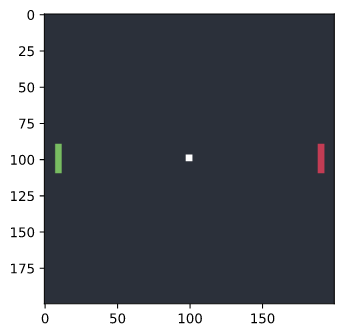
\includegraphics[scale=0.53]{figures/raw.png}
        \caption{Raw 200x200 frame}
        \label{fig-raw}
    \end{subfigure}
    \begin{subfigure}{0.49\textwidth}
        \centering
        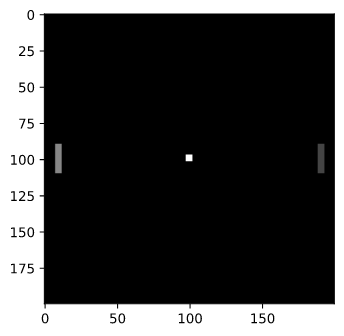
\includegraphics[scale=0.53]{figures/bw.png}
        \caption{Black and White processed frame}
        \label{fig-bw}
    \end{subfigure}

    \begin{subfigure}{0.49\textwidth}
        \centering
        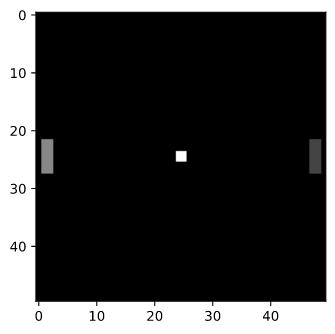
\includegraphics[scale=0.53]{figures/small.png}
        \caption{Down Sampled 50x50 frame}
    \end{subfigure}
    \caption{Frame in different stages of processing}
    \label{fig-small}
    \label{fig-process}
\end{figure}

\pagebreak